\section{Project Description} \label{sec:project_description}
The objective of this project was to implement a 16-bit Kogge-Stone Adder in \SI{0.35}{\micro\m} technology which from now on will be called KS adder. The KS adder belongs to the family of parallel-prefix adders which reduces the critical path compared to regular ripple-carry adders. The cost for this is paid in area and complex routing which prolongs development time.

Fast adders are very important in all types of integrated circuits since almost all algorithms one can come up with consists of at least one addition. 

The official goal was to reach a speed of \SI{200}{\mega\Hz} but the group decided on an unofficial goal to reach a speed of \SI{400}{\mega\Hz}.

\begin{figure}[H]
  \centering
  \captionsetup{justification=centering}
  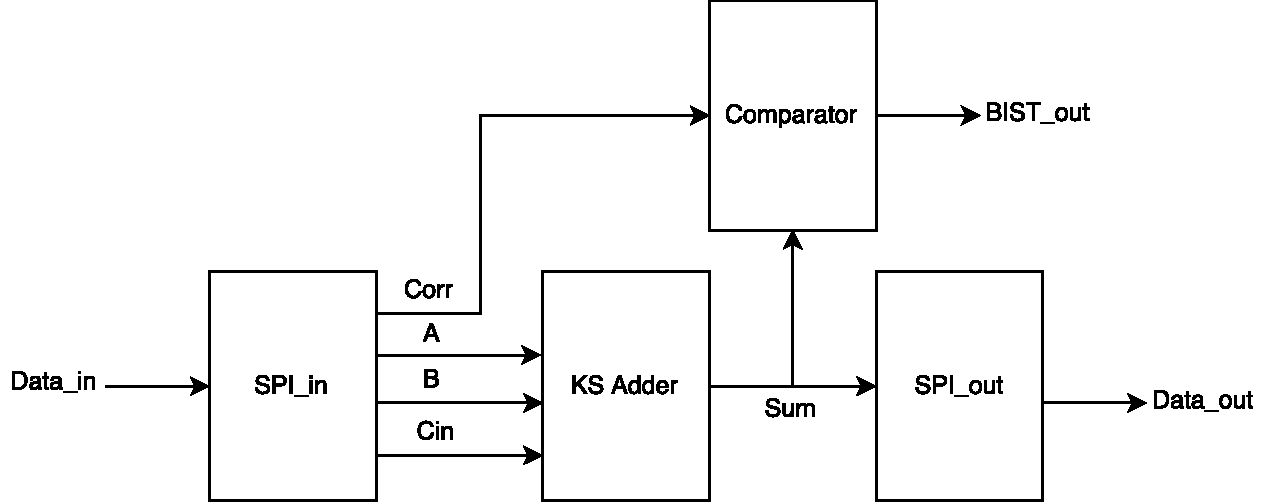
\includegraphics[scale=0.5]{../figures/TOP.pdf}
  \caption{Block diagram of the system after first iteration.} \label{fig:block_first}
\end{figure}

\begin{figure}[H]
\centering
\captionsetup{justification=centering}
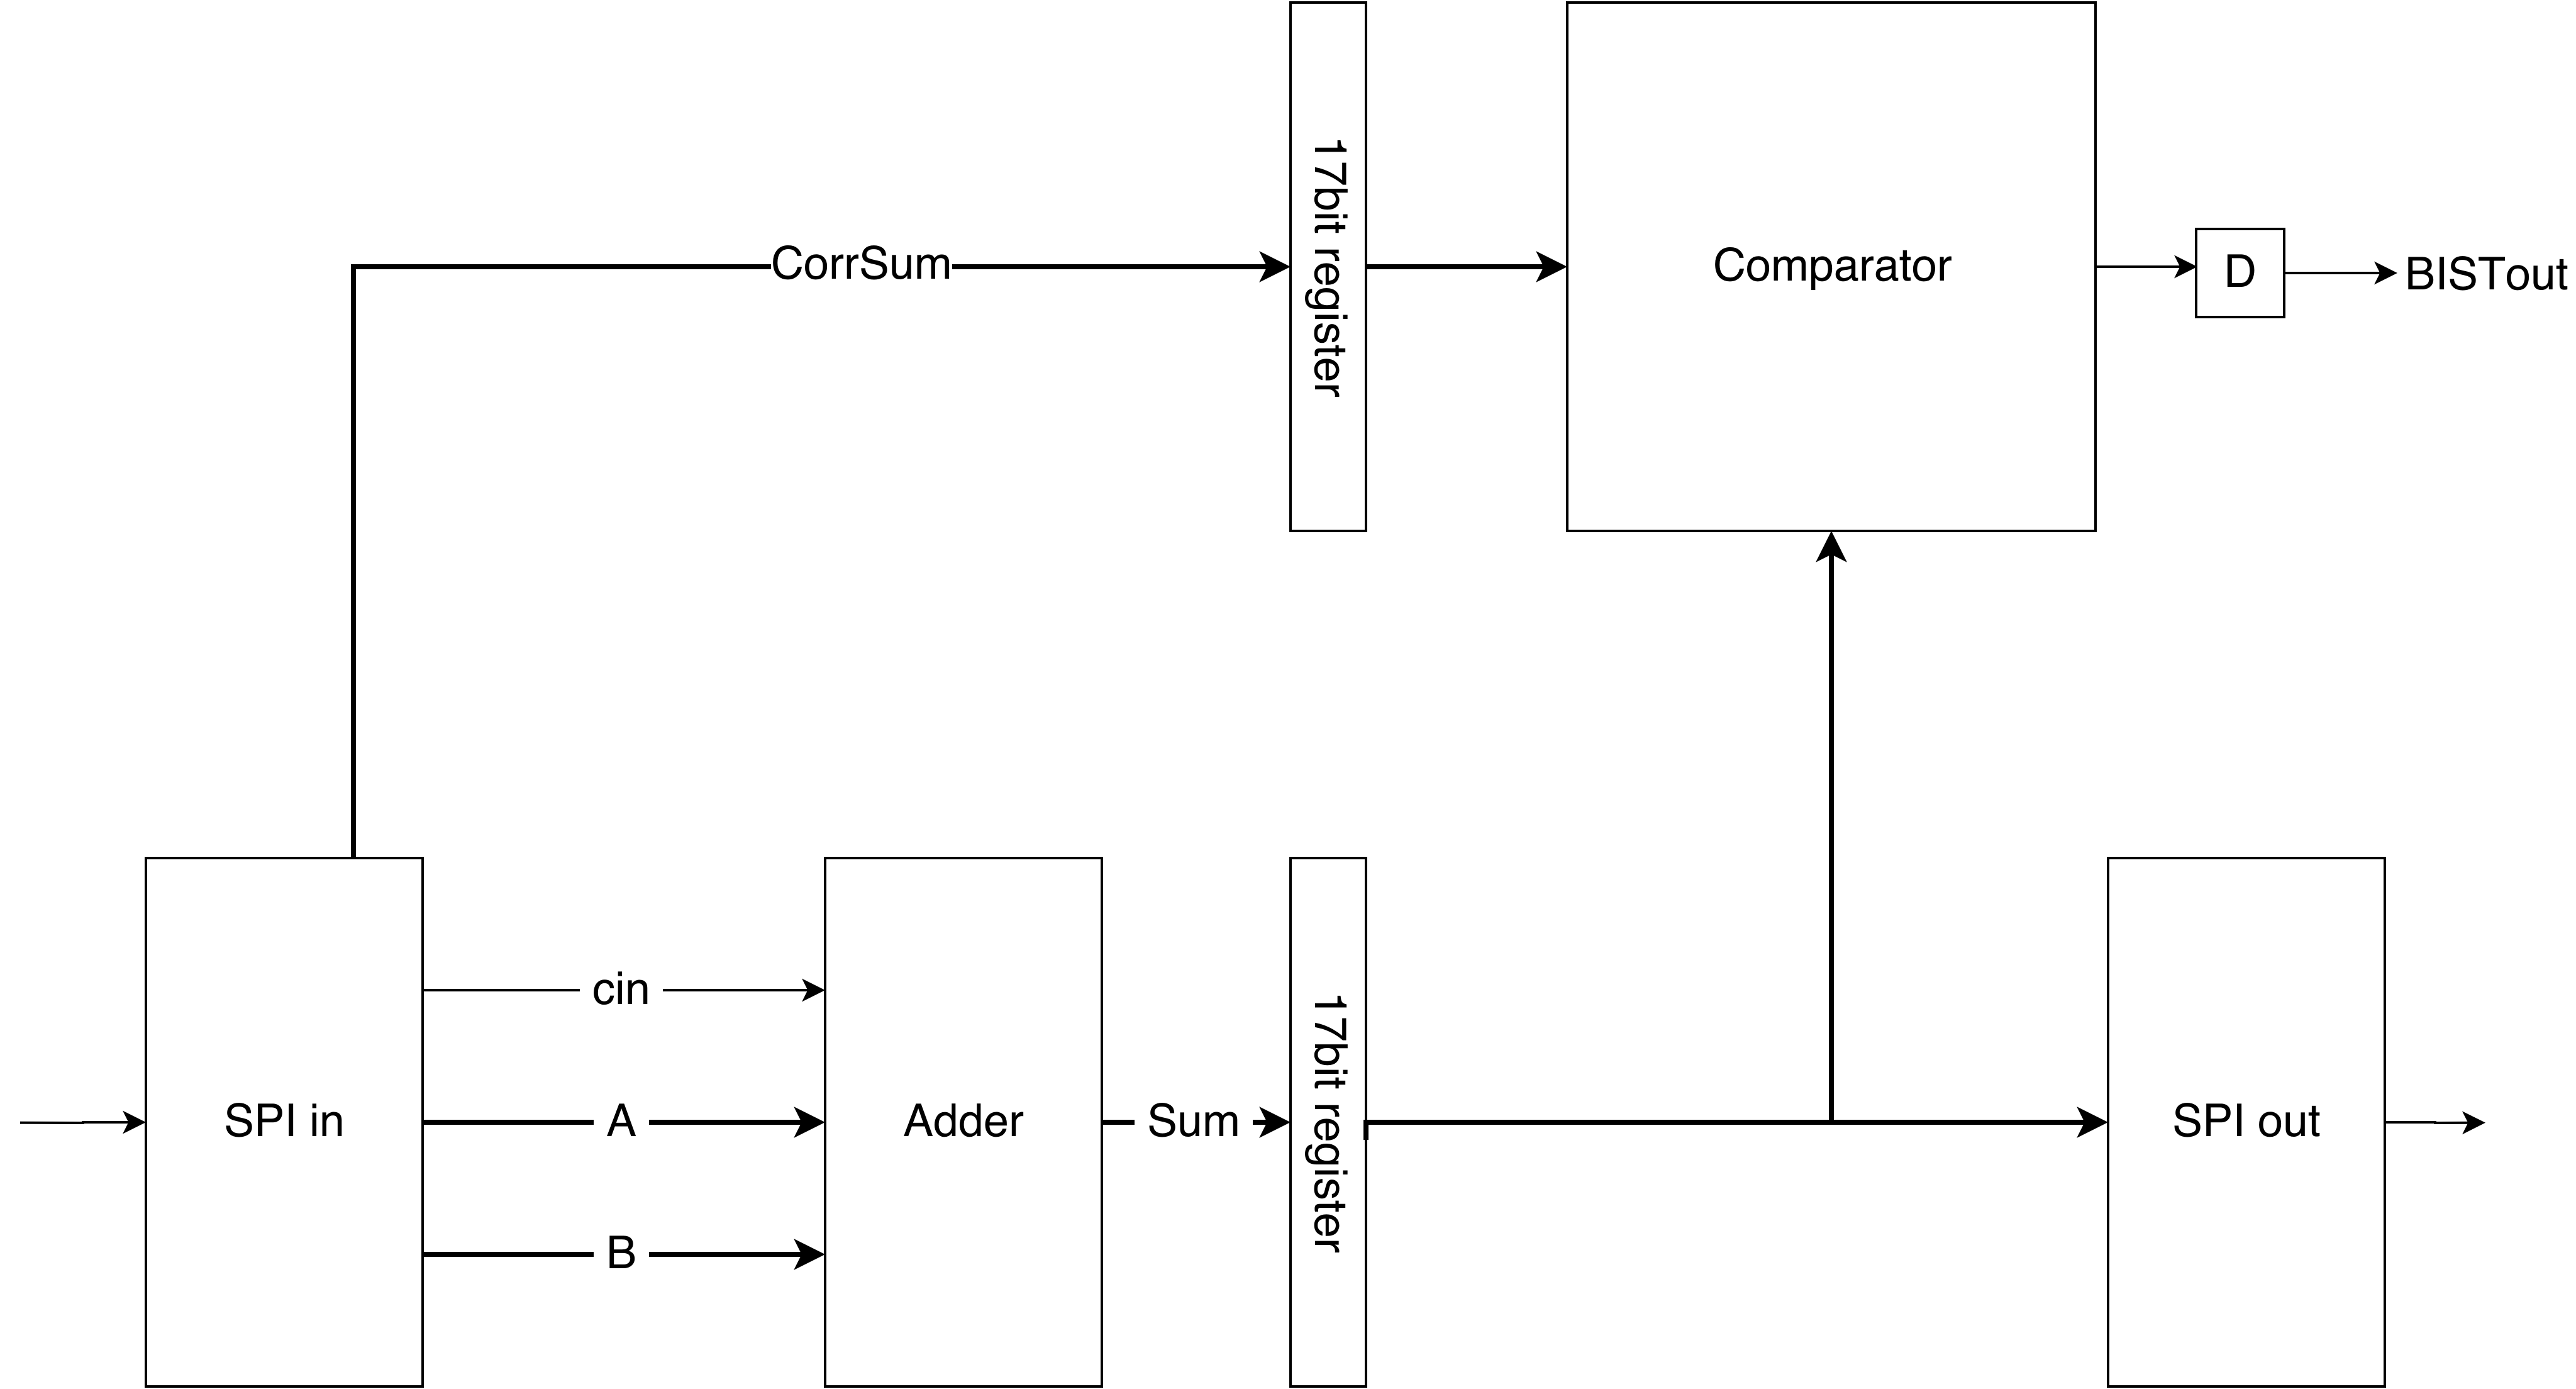
\includegraphics[scale=0.1]{../figures/top_level_second.png}
\caption{Block diagram of the system after second iteration.} \label{fig:block_second}
\end{figure}

\begin{figure}[H]
\centering
\captionsetup{justification=centering}
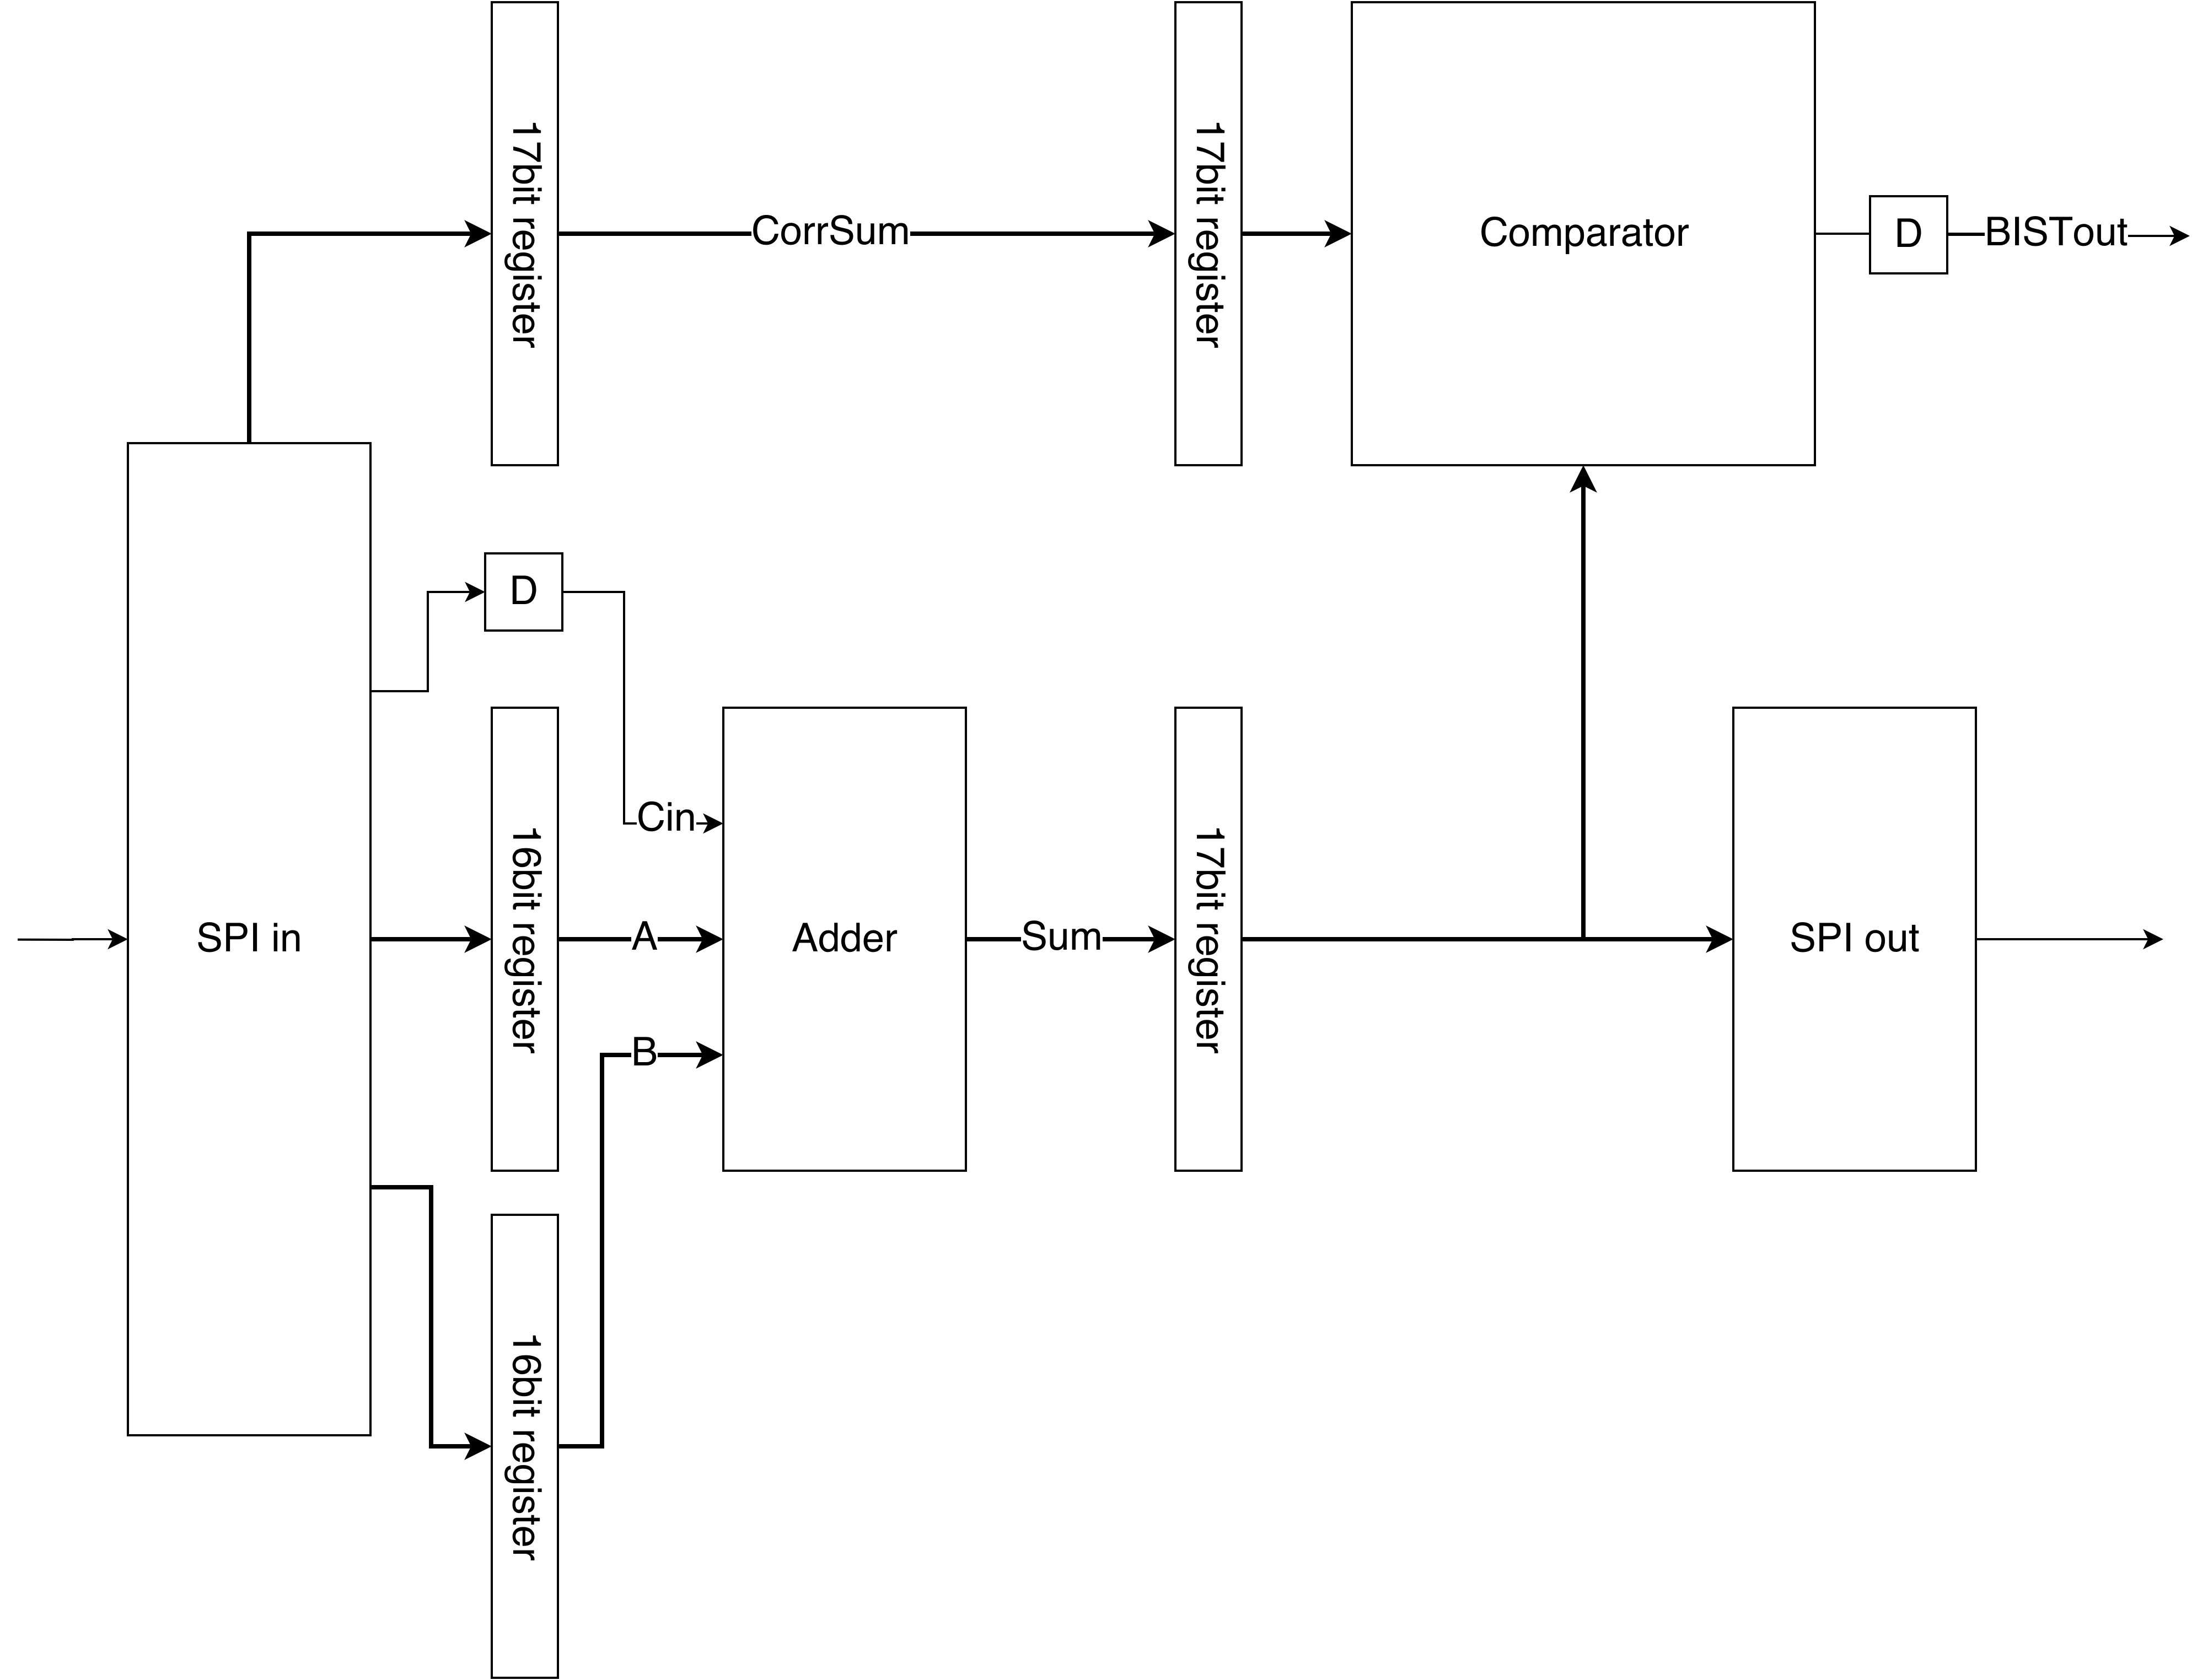
\includegraphics[scale=0.1]{../figures/top_level_final.png}
\caption{Final block diagram of the system.}  \label{fig:block_final}
\end{figure}

In Fig. \ref{fig:block_first} the block diagram of the system after the first design phase is depicted. One can note that the signal goes from one block to the next directly. In Fig. \ref{fig:block_second} some registers have been introduced to make sure BISTout stays the same between clock pulses when new data is evaluated and to give a more stable signal to the comparator and SPI-out unit. In the final iteration additional register have been inserted between SPI in and the adder to cut the path from the registers in the SPI unit to the adder and to make sure that all bits in the same word arrives at the same time to the adder. The block diagram from the last iteration can be seen in Fig. \ref{fig:block_final}.

\subsection{SPI-in}
The SPI-in module is supposed to serially receive four times four 16-bit numbers and to distribute these to the correct parts of the system. 

\subsubsection{SPI-recieve}
The first part in the SPI-in module is SPI-receive, where we receive all the bits (see figure \ref{fig:spi_receive}). It consists of 16 D flip-flops (DFF), that is connected one after another in a serial manner. They are clocked on the SPI clock, and on each positive clock edge, a new input bit is shifted in. After 16 pulses we have 16 bits stored, and a load signal is triggered so that each bit is moved to the correct test-register.

\begin{figure}[H]
	\centering
	\captionsetup{justification=centering}
	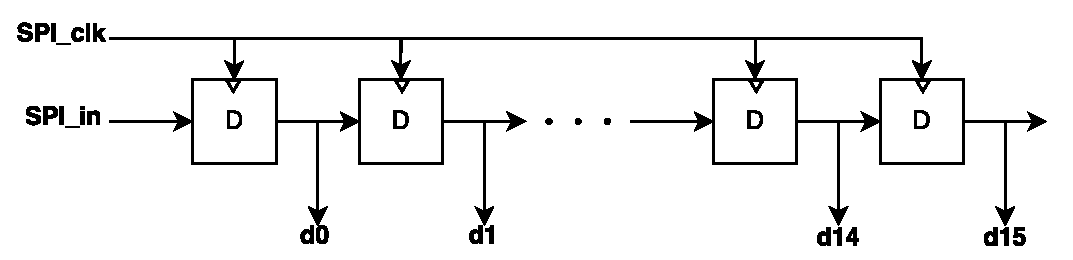
\includegraphics[scale=0.5]{../figures/SPI_receive.pdf}
	\caption{Block diagram of the SPI-receive block.} \label{fig:spi_receive}
\end{figure}

\subsubsection{Test-registers}
The test-registers (see Fig. \ref{fig:spi_prbs}) consists of four flip flops (one for each addition). While SPI\_enable is low, we load the registers with data from SPI-receive, and when it is high one of two thing can happen, depending on what we want to test. If we want to test the energy consumption, then the new data to the registers are pseudo-random data, that we get from a XOR of the third and fourth bit in the register, meaning we get 16 different values. And if we want to test the speed, then the same data is looped through the registers over and over, meaning we can slowly increase the clock rate and see when the system produces the wrong data.

\begin{figure}[H]
	\centering
	\captionsetup{justification=centering}
	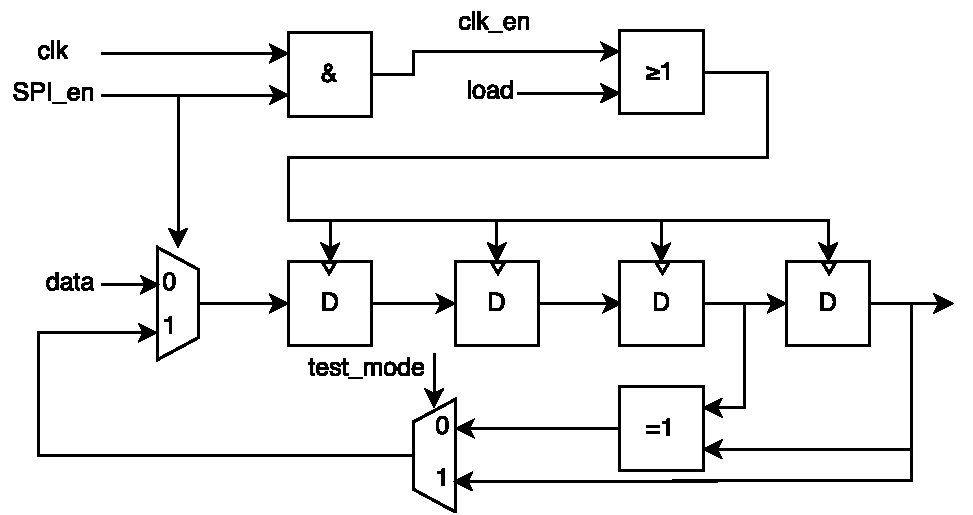
\includegraphics[scale=0.5]{../figures/SPI_PRBS_2.pdf}
	\caption{Block diagram of the test-registers.} \label{fig:spi_prbs}
\end{figure}

\subsubsection{SPI-controller}
The last part of this module is some control logic (see Fig. \ref{fig:spi_controller}). The heart of the control block is a 6-bit counter, where the first four bits signalizes if we have read a 16 bit word or not and the last two bits signalizes which of our four words we are currently reading. By combining these signals like in the figure we are able to produce the load signals that trigger the test-registers.

\begin{figure}[H]
	\centering
	\captionsetup{justification=centering}
	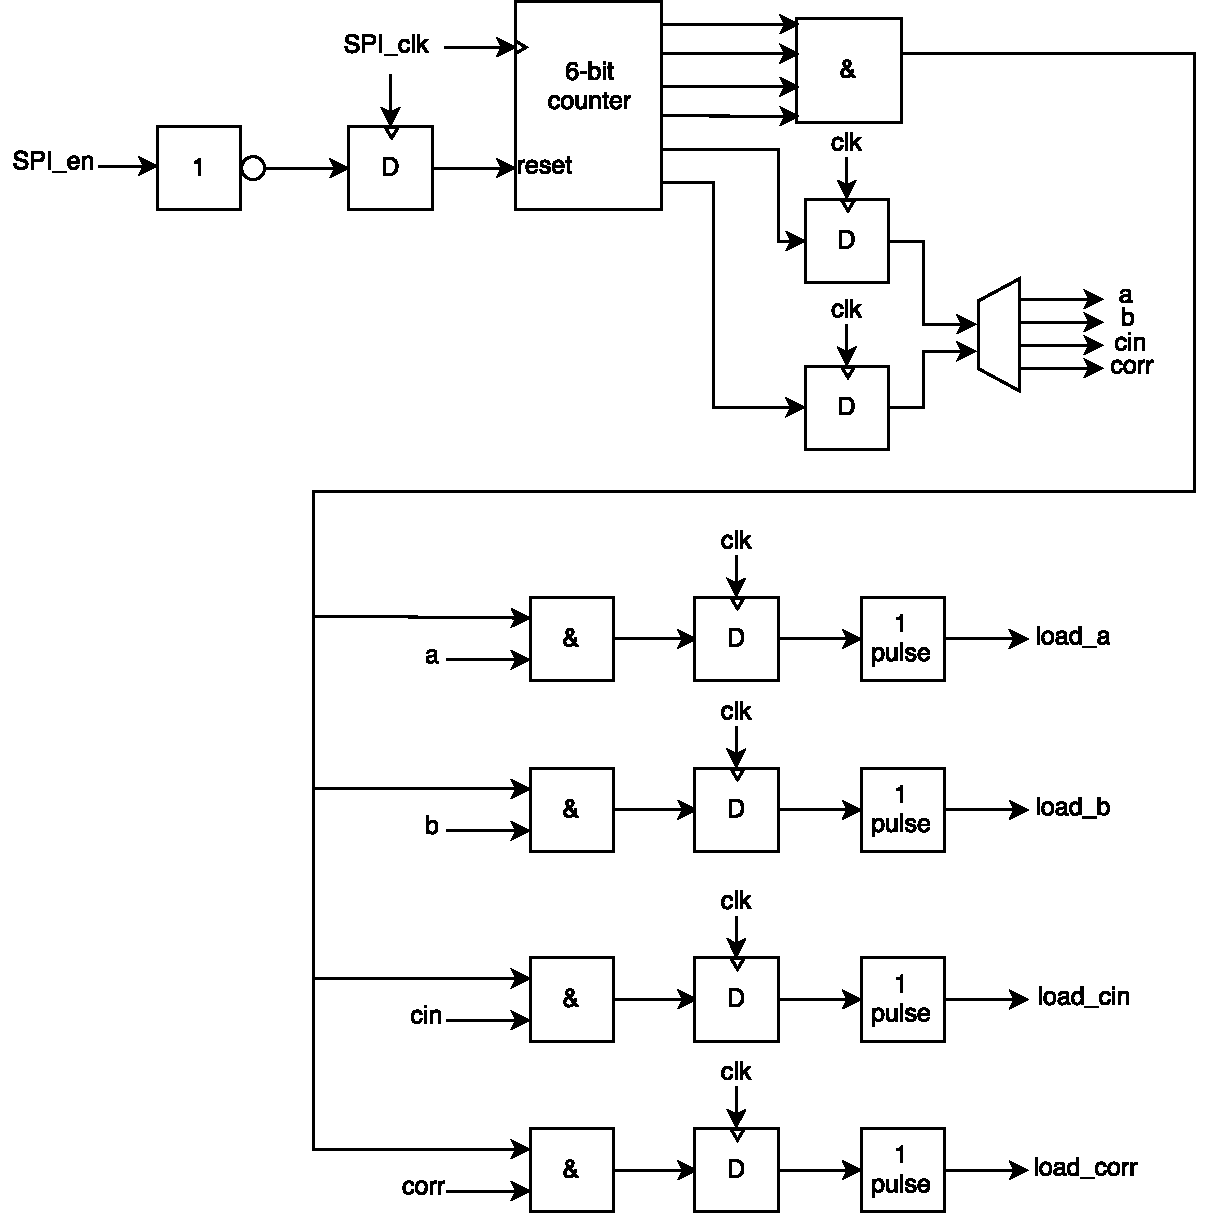
\includegraphics[scale=0.5]{../figures/SPI_controller.pdf}
	\caption{Block diagram of the SPI-controller.} \label{fig:spi_controller}
\end{figure}

\subsection{16-bit Kogge-Stone Adder}
The KS adder consists of several simple blocks connected in a complex way. The \textit{yellow} block has been split into two blocks \textit{yellow\_inv\_in} and \textit{yellow\_inv\_out}, which can be seen in Fig. \ref{fig:yellow_opt}. The \textit{yellow\_inv\_in} block takes inverted input signals and gives non-inverted output. The \textit{yellow\_inv\_out} block takes non-inverted inputs and gives inverted output. This arrangement saves a lot of gates. The \textit{yellow\_carry} block has been split in the same way. 

Because of the inverted signals from \textit{yellow\_inv\_out} some \textit{sum} blocks have been replaced with XNOR gates instead of XOR gates which are the case in a standard KS adder design. A couple of inverters have also been added within the adder to make sure the new blocks gets the correct input.

\begin{figure}[H]
  \centering
  \captionsetup{justification=centering}
  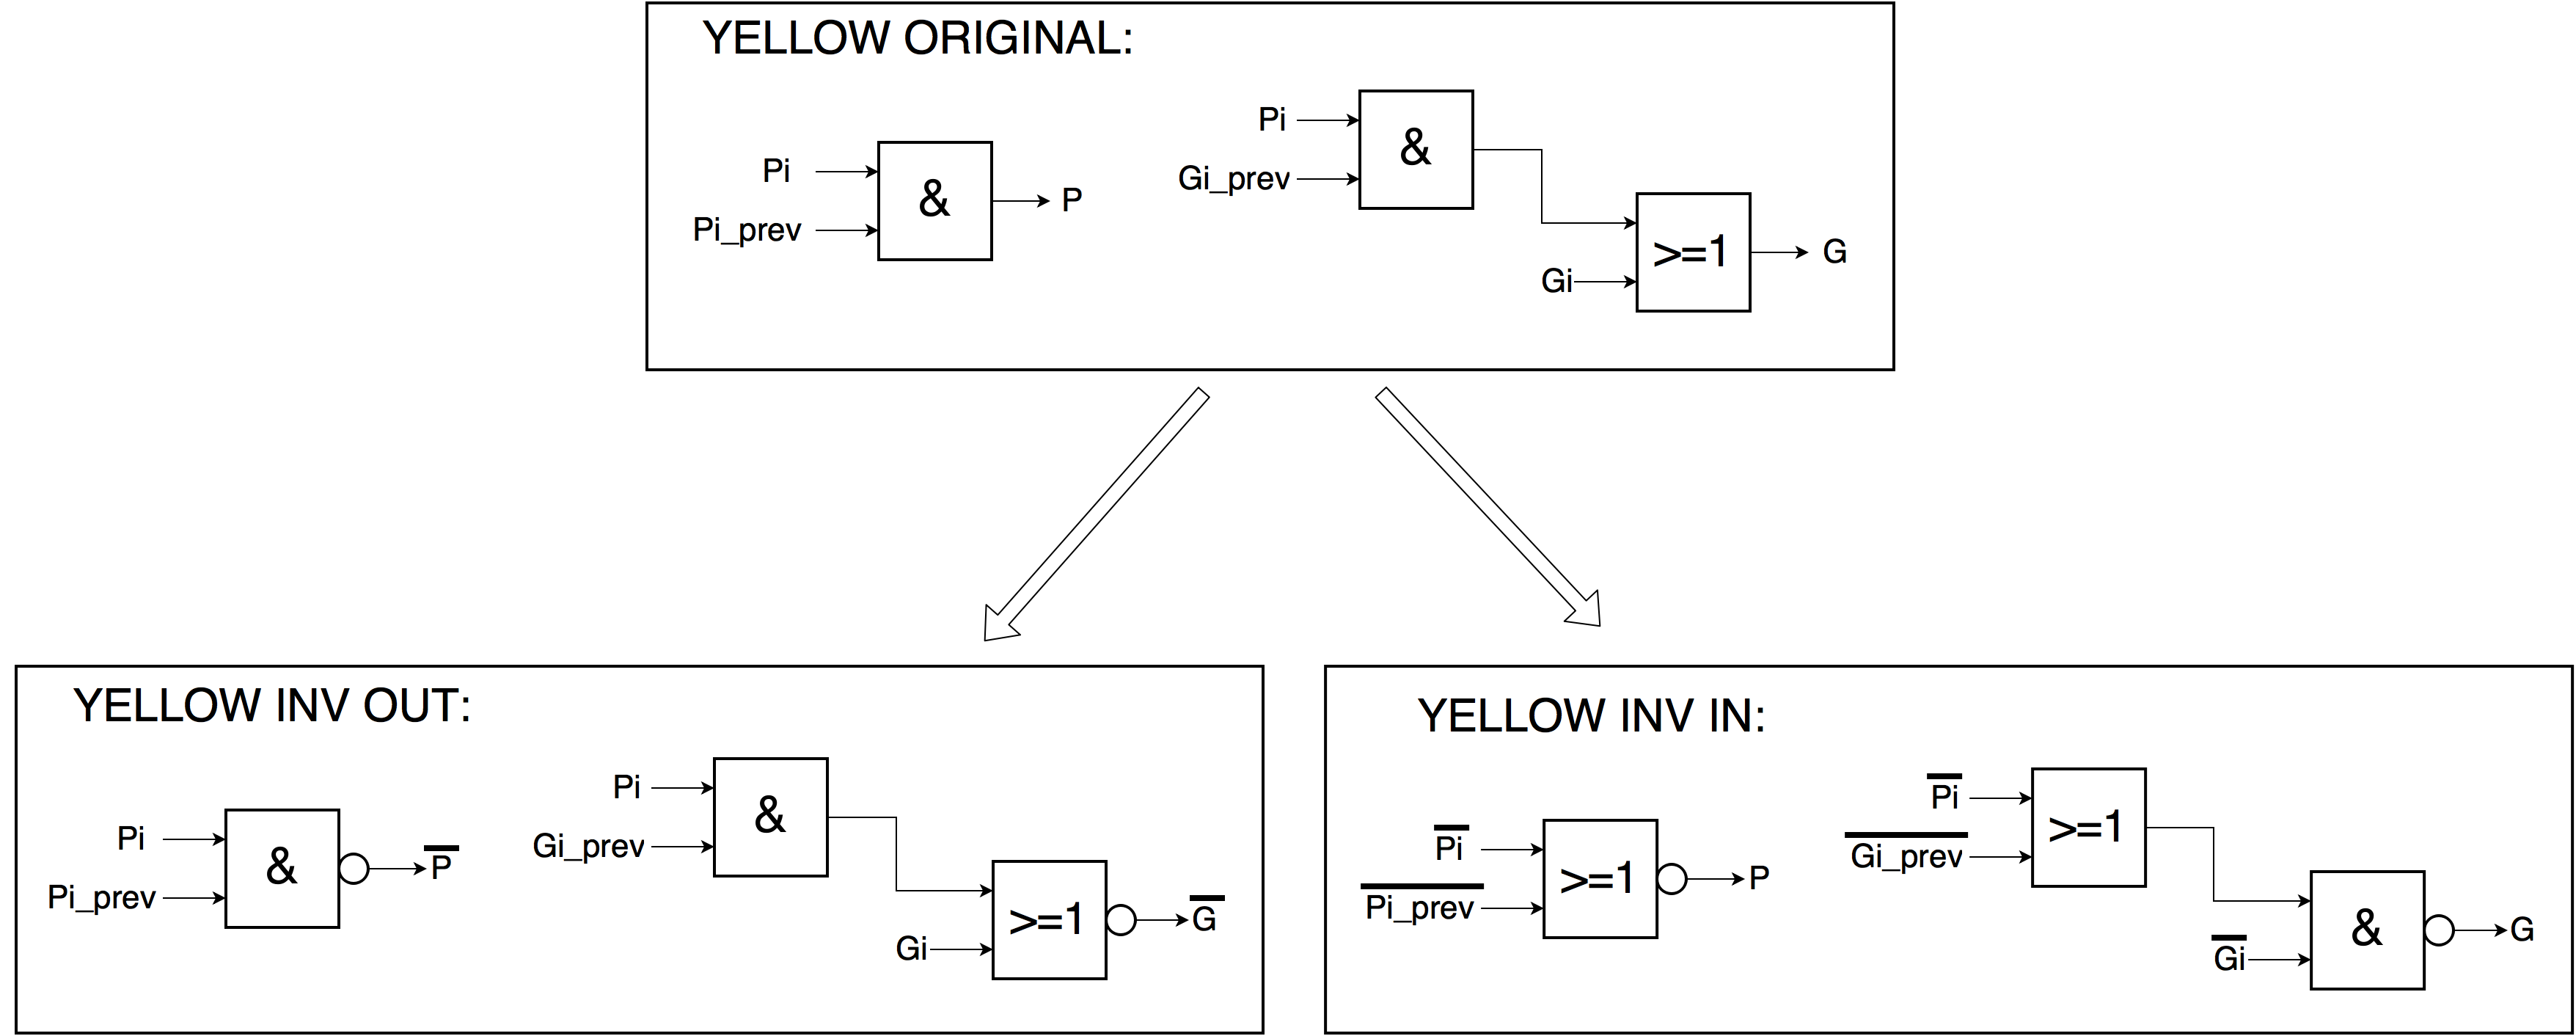
\includegraphics[scale=0.12]{../figures/yellow_opt}
  \caption{The new yellow blocks.} \label{fig:yellow_opt}
\end{figure}

To save space, new switch nets were created for the generate calculation of the \textit{yellow} blocks. The new nets can be seen in Fig. \ref{fig:G_inv_in} and \ref{fig:G_inv_out}. By doing this the transistor count is cut in half. 

\begin{figure}[H]
  \centering
  \captionsetup{justification=centering}
  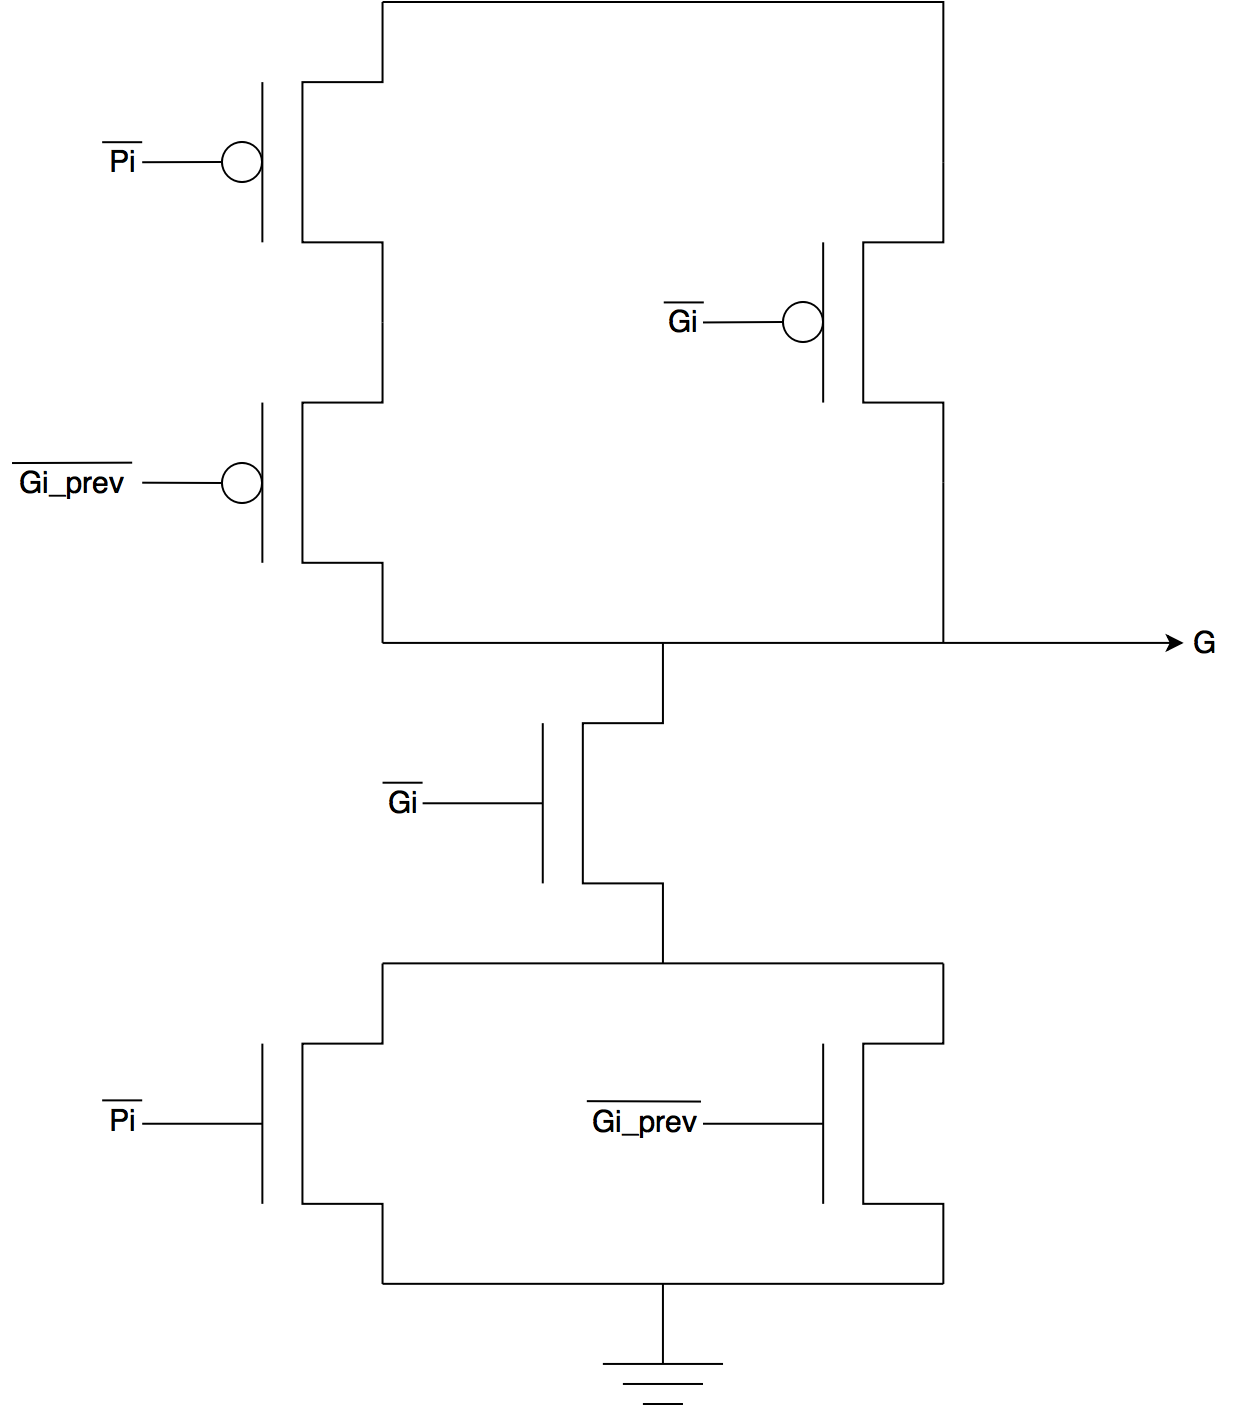
\includegraphics[scale=0.15]{../figures/G_inv_in}
  \caption{Generate part of \textit{yellow\_inv\_in}.} \label{fig:G_inv_in}
\end{figure}

\begin{figure}[H]
  \centering
  \captionsetup{justification=centering}
  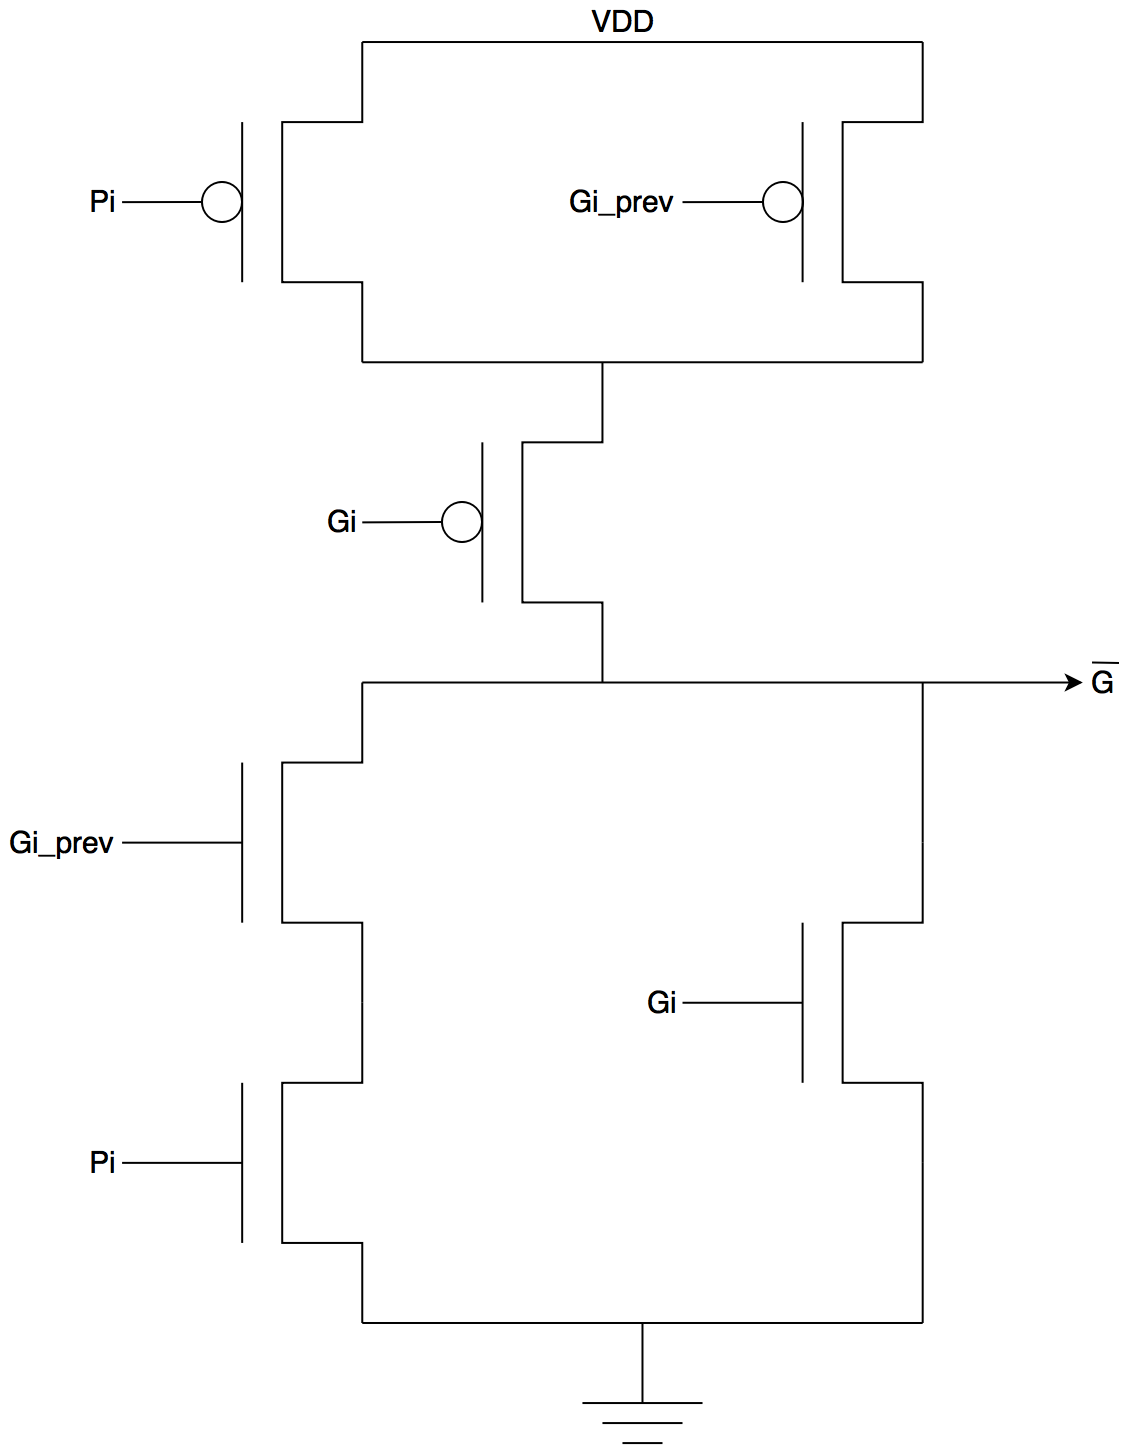
\includegraphics[scale=0.15]{../figures/G_inv_out}
  \caption{Generate part of \textit{yellow\_inv\_out}.} \label{fig:G_inv_out}
\end{figure}

\subsection{SPI-out}